\documentclass[11pt]{article}
\usepackage[spanish]{babel}
\usepackage{amsmath, amssymb, bm}
\usepackage[a4paper,margin=2.5cm]{geometry}
\usepackage{graphicx}
\usepackage{hyperref}
\usepackage{float}


\newcommand{\ii}{\mathrm{i}}

\usepackage{titling}
\pretitle{\begin{center}\LARGE\bfseries}
\posttitle{\end{center}}
\title{Apuntes Quantum}
\author{
    Lukas Wolff}
\date{}

\begin{document}
\maketitle

\section{Qubit}

Un qubit se puede definir como:

\begin{equation}
    |\psi\rangle = \alpha |0\rangle + \beta |1\rangle
\end{equation}

Donde se debe cumplir por probabilidad que:

\begin{equation}
    |\alpha|^2 + |\beta|^2 = 1
\end{equation}

Ahora bien, se puede tener una superposicion de 2 o mas qubits, por ejemplo:

\begin{equation}
    |\psi\rangle = \alpha |00\rangle + \beta |01\rangle + \gamma |10\rangle + \delta |11\rangle
\end{equation}

Por lo tanto, el espacio lineal de n qubits es:

\begin{equation}
    |\psi\rangle = \sum_{}^{} \alpha_i |i\rangle
\end{equation}

\subsection{Angulos del qubit}

Un qubit se puede representar en una esfera de radio 1, conocida como esfera de Bloch. Para esto, se definen dos angulos $\theta$ y $\phi$:

\begin{equation}
    |\psi\rangle = \cos\left(\frac{\theta}{2}\right) |0\rangle + e^{\ii \phi} \sin\left(\frac{\theta}{2}\right) |1\rangle
\end{equation}

Donde, recordar que se un numero imaginario $a + bi$, se puede definiri como:

\begin{equation}
    a + bi = re^{\ii \phi} \quad \text{con} \quad r = \sqrt{a^2 + b^2} \quad \text{y} \quad \phi = \tan^{-1}\left(\frac{b}{a}\right)
\end{equation}

Donde los angulos en la esfera de Bloch se visualizan como:

\begin{figure}[H]
    \centering
    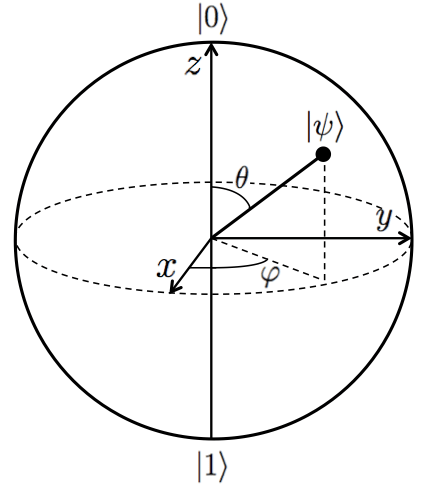
\includegraphics[width=0.3\textwidth]{ANGULOS.png}
    \caption{Esfera de Bloch}
    \label{fig:bloch_sphere}
\end{figure}


\subsection{Bases}

Las bases son conjuntos de qubits ortogonales entre si, que permiten representar cualquier qubit como una combinacion lineal de los qubits de la base. Algunas bases comunes son:

\begin{equation}
    |0\rangle = \begin{pmatrix} 1 \\ 0 \end{pmatrix}, \quad |1\rangle = \begin{pmatrix} 0 \\ 1 \end{pmatrix}
\end{equation}

\begin{equation}
    |+\rangle = \frac{1}{\sqrt{2}} (|0\rangle + |1\rangle) = \frac{1}{\sqrt{2}} \begin{pmatrix} 1 \\ 1 \end{pmatrix}, \quad |-\rangle = \frac{1}{\sqrt{2}} (|0\rangle - |1\rangle) = \frac{1}{\sqrt{2}} \begin{pmatrix} 1 \\ -1 \end{pmatrix}
\end{equation}

\begin{equation}
    |+y\rangle = \frac{1}{\sqrt{2}} (|0\rangle + \ii |1\rangle) = \frac{1}{\sqrt{2}} \begin{pmatrix} 1 \\ \ii \end{pmatrix}, \quad |-y\rangle = \frac{1}{\sqrt{2}} (|0\rangle - \ii |1\rangle) = \frac{1}{\sqrt{2}} \begin{pmatrix} 1 \\ -\ii \end{pmatrix}
\end{equation}

\subsection{Producto tensorial}

El producto tensorial permite combinar dos o mas qubits para formar un sistema de qubits. Si se tienen dos qubits $|\psi\rangle$ y $|\phi\rangle$, definidos como:

\begin{equation}
    |\psi\rangle = \begin{pmatrix} v_1 \\ v_2 \end{pmatrix}, \quad |\phi\rangle = \begin{pmatrix} w_1 \\ w_2 \end{pmatrix}
\end{equation}

El producto tensorial entre ambos qubits es:

\begin{equation}
    |\psi\rangle \otimes |\phi\rangle = \begin{pmatrix} v_1 w_1 \\ v_1 w_2 \\ v_2 w_1 \\ v_2 w_2 \end{pmatrix} = v_1 w_1 |00\rangle + v_1 w_2 |01\rangle + v_2 w_1 |10\rangle + v_2 w_2 |11\rangle
\end{equation}

\section{Dual}

Sea un qubit base:

\begin{equation}
    |\psi\rangle = \begin{pmatrix} \alpha \\ \beta \end{pmatrix} = \alpha |0\rangle + \beta |1\rangle
\end{equation}

El dual de este qubit es:

\begin{equation}
    \langle \psi | = \begin{pmatrix} \alpha^* & \beta^* \end{pmatrix} = \alpha^* \langle 0| + \beta^* \langle 1|
\end{equation}

Donde la notacion $^*$ denota el conjugado complejo, es decir, si $\alpha = a + bi$, entonces $\alpha^* = a - bi$. El espacio lineal de los duales es:

\begin{equation}
    \langle \psi | = \sum_{}^{} \alpha_i^* \langle i |
\end{equation}

\section{Producto interno escalar o bra-ket}

Sea el qubit:

\begin{equation}
    |\psi\rangle = \begin{pmatrix} v_1 \\ v_2 \end{pmatrix}
\end{equation}

Y el dual:

\begin{equation}
    \langle \phi | = \begin{pmatrix} w_1^* & w_2^* \end{pmatrix}
\end{equation}

El producto interno escalar entre un qubit y un dual es:

\begin{equation}
    \langle \phi | \psi \rangle = \sum_{i} w_i^* v_i = w_1^* v_1 + w_2^* v_2
\end{equation}

Donde se cumple que:

\begin{equation}
    \langle \phi | \psi \rangle = \langle \psi | \phi \rangle^*
\end{equation}

Si dos vectores son ortogonales, se cumple que:

\begin{equation}
    \langle \phi | \psi \rangle = 0
\end{equation}

Y si es un vector consigo mismo, se cumple que:

\begin{equation}
    \langle \psi | \psi \rangle = 1
\end{equation}

\section{Producto externo o ket-bra}

Sea el qubit:

\begin{equation}
    |\psi\rangle = \begin{pmatrix} v_1 \\ v_2 \end{pmatrix}
\end{equation}

Y el dual:

\begin{equation}
    \langle \phi | = \begin{pmatrix} w_1^* & w_2^* \end{pmatrix}
\end{equation}

El producto externo entre un qubit y un dual es:

\begin{equation}
    |\psi\rangle \langle \phi | = \begin{pmatrix} v_1 w_1^* & v_1 w_2^* \\ v_2 w_1^* & v_2 w_2^* \end{pmatrix}
\end{equation}

Lo cual es la matriz de proyeccion del qubit $|\psi\rangle$ sobre el dual $\langle \phi |$.

Luego, para cualquier base se cumple que:

\begin{equation}
    I = \sum_{i} |i\rangle \langle i |
\end{equation}

Donde $I$ es el operador identidad, por ejemplo, para la base computacional:

\begin{equation}
    I = |0\rangle \langle 0| + |1\rangle \langle 1| = \begin{pmatrix} 1 & 0 \\ 0 & 0 \end{pmatrix} + \begin{pmatrix} 0 & 0 \\ 0 & 1 \end{pmatrix} = \begin{pmatrix} 1 & 0 \\ 0 & 1 \end{pmatrix}
\end{equation}

\section{Operadores}

Los operadores son matrices que actuan sobre los qubits, generando una rotacion del estado, o una transformacion del mismo. Algunos operadores basicos son:

\begin{itemize}
    \item Operador identidad:
    \begin{equation}
        I = \begin{pmatrix} 1 & 0 \\ 0 & 1 \end{pmatrix}
    \end{equation}
    
    \item Operador X (NOT):
    \begin{equation}
        X = \begin{pmatrix} 0 & 1 \\ 1 & 0 \end{pmatrix}
    \end{equation}
    
    \item Operador Y:
    \begin{equation}
        Y = \begin{pmatrix} 0 & -\ii \\ \ii & 0 \end{pmatrix}
    \end{equation}
    
    \item Operador Z:
    \begin{equation}
        Z = \begin{pmatrix} 1 & 0 \\ 0 & -1 \end{pmatrix}
    \end{equation}
    
    \item Operador Hadamard:
    \begin{equation}
        H = \frac{1}{\sqrt{2}} \begin{pmatrix} 1 & 1 \\ 1 & -1 \end{pmatrix}
    \end{equation}
\end{itemize}

\subsection{Operador NOT de una base cualquiera}

Para calcular el operador NOT de una base cualquiera, se debe conocer los vectores de la base. Sea la base:

\begin{equation}
    |u\rangle = \begin{pmatrix} a \\ b \end{pmatrix}, \quad |v\rangle = \begin{pmatrix} c \\ d \end{pmatrix}
\end{equation}

El operador NOT en esta base se define como:

\begin{equation}
    X_{uv} = |u\rangle \langle v| + |v\rangle \langle u| = \begin{pmatrix} a \\ b \end{pmatrix} \begin{pmatrix} c^* & d^* \end{pmatrix} + \begin{pmatrix} c \\ d \end{pmatrix} \begin{pmatrix} a^* & b^* \end{pmatrix}
\end{equation}

\subsection{Operador unitario}

Un operador unitario es aquel que cumple que:

\begin{equation}
    U^\dagger U = U U^\dagger = I
\end{equation}

Donde $U^\dagger$ es el conjugado transpuesto de $U$. Los operadores unitarios son importantes en la mecanica cuantica, ya que representan las transformaciones que pueden sufrir los estados cuanticos sin perder informacion. Se cumple que:

\begin{equation}
    \langle \psi | U^\dagger U | \psi \rangle = \langle \psi | I | \psi \rangle = \langle \psi | \psi \rangle = 1
\end{equation}

\subsection{Operaciones}

La operacion de un operador sobre un qubit se representa como:

\begin{equation}
    |\psi\rangle \rightarrow U = U |\psi\rangle
\end{equation}

\section{Entrelazamiento}

El entrelazamiento es un fenomeno cuantico que ocurre cuando dos o mas qubits estan correlacionados de tal manera que el estado de uno depende del estado del otro, incluso si estan separados por grandes distancias. Un ejemplo comun de un estado entrelazado es el estado de Bell:

\begin{equation}
    |\Phi^+\rangle = \frac{1}{\sqrt{2}} (|00\rangle + |11\rangle)
\end{equation}

Es decir, si se mide el primer qubit y se obtiene 0, el segundo qubit tambien sera 0. Si se mide el primer qubit y se obtiene 1, el segundo qubit tambien sera 1.

Es importante notar que una vez que se genera entrelazamiento, no se puede deshacer mediante operaciones locales en los qubits individuales.

\subsection{Regla de CHSH}

La desigualdad de CHSH es una extension de la desigualdad de Bell, que permite cuantificar el grado de entrelazamiento entre dos qubits. Se define como:

\begin{equation}
    S = E(a, b) - E(a, b') + E(a', b) + E(a', b')
\end{equation}

Donde $E(a, b)$ es la correlacion entre las mediciones de los qubits en las direcciones $a$ y $b$. Si se encuentra que $|S| > 2$, entonces los qubits estan entrelazados con un limite superior de $|S| \leq 2\sqrt{2}$.

\subsection{Teorema de no clonacion}

El teorema de no clonacion establece que no es posible crear una copia exacta de un estado cuantico desconocido. Esto se debe a que la operacion de clonacion violaria los principios fundamentales de la mecanica cuantica, como la superposicion y el entrelazamiento. 

Demostracion por contradiccion, sea U el copiador universal, entonces se debe cumplir que:

\begin{equation}
    U |\psi\rangle |0\rangle = |\psi\rangle |\psi\rangle \quad (1)
\end{equation}

\begin{equation}
    U |\psi\rangle |0\rangle = \alpha^2 |0\rangle |0\rangle + \alpha \beta |0\rangle |1\rangle + \alpha \beta |1\rangle |0\rangle + \beta^2 |1\rangle |1\rangle \quad (2)
\end{equation}

Pero tal operacion debe ser cierta para cualquier estado, por lo que si lo aplicamos a la base:

\begin{equation}
    U |0\rangle |0\rangle = |0\rangle |0\rangle \quad 
\end{equation}

Analogo para el estado $|1\rangle$:

\begin{equation}
    U |1\rangle |0\rangle = |1\rangle |1\rangle \quad
\end{equation}

Usando propiedades lineales, sabemos que:

\begin{equation}
    U |\psi\rangle = U (\alpha |0\rangle + \beta |1\rangle) 
\end{equation}

Por lo tanto:

\begin{equation}
    U (\alpha |0\rangle + \beta |1\rangle) |0\rangle = \alpha |0\rangle |0\rangle + \beta |1\rangle |1\rangle \quad (3)
\end{equation}

Donde es aplicada la misma logica que la copia de un estado clasico. Pero si comparamos (2) y (3), vemos que no son iguales, por lo que se llega a una contradiccion, y por lo tanto, no es posible clonar un estado cuantico desconocido.

\section{Ejercicos resueltos}

\end{document}